\subsection{Designing a Beverage Antenna for Success!}
\begin{tcolorbox}[colback=gray!10, colframe=black, title=E9H01]
When constructing a Beverage antenna, which of the following factors should be included in the design to achieve good performance at the desired frequency?
\begin{enumerate}[label=\Alph*.]
    \item Its overall length must not exceed 1/4 wavelength
    \item It must be mounted more than 1 wavelength above ground
    \item It should be configured as a four-sided loop
    \item \textbf{It should be at least one wavelength long}
\end{enumerate} \end{tcolorbox}

\subsubsection{Understanding Beverage Antennas}
A Beverage antenna is a type of long-wire receiving antenna used in radio communication, typically for low-frequency bands. When designing such antennas, one must consider several key factors to ensure good performance.

\subsubsection{Key Design Factors}
The correct answer to the question is that the Beverage antenna should be at least one wavelength long. This aspect of its design is crucial for several reasons:

1. \textbf{Length Requirement:}: The effective length of the antenna is pivotal because it determines the antenna's efficiency at receiving signals. A length of at least one wavelength ensures that the antenna can efficiently couple with the electromagnetic waves of the target frequency.

2. \textbf{Performance Characteristics:}: Antenna length plays a vital role in its directivity and gain. A longer antenna can provide better directivity, helping to minimize the noise and improve the reception of weak signals from a specific direction.

3. \textbf{Operational Frequency:}: The operational frequency of an antenna is directly related to its length. The relationship can be expressed mathematically as:
   \[
   L = \frac{c}{f}
   \]
   where \( L \) is the length of the antenna (in meters), \( c \) is the speed of light in a vacuum (\( \approx 3 \times 10^8 \) m/s), and \( f \) is the frequency (in Hz).

\subsubsection{Example Calculation}
For example, if the desired operational frequency is 3.5 MHz, the length of the antenna can be calculated as follows:
\[
f = 3.5 \times 10^6 \text{ Hz}
\]
\[
L = \frac{3 \times 10^8 \text{ m/s}}{3.5 \times 10^6 \text{ Hz}} \approx 85.71 \text{ meters}
\]
This result indicates that for best performance, the Beverage antenna should exceed this length to fully utilize its potential in receiving the designated frequency signals.

\subsubsection{Conclusion}
To summarize, when constructing a Beverage antenna, it is essential to ensure that it is at least one wavelength long for optimal performance at the desired frequency. This consideration enhances the antenna's ability to receive signals effectively. Additionally, while other factors, such as height above ground and configuration, are important, they do not overshadow the significance of antenna length.

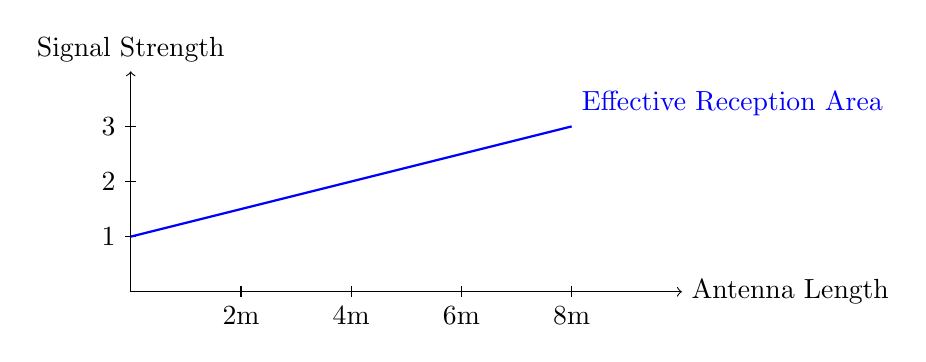
\begin{tikzpicture}[scale=0.7]
    \draw[->] (0,0) -- (10,0) node[right] {Antenna Length};
    \draw[->] (0,0) -- (0,4) node[above] {Signal Strength};
    \foreach \x in {2, 4, 6, 8} {
        \draw (\x,0.1) -- (\x,-0.1) node[below] {\x m};
    }
    \foreach \y in {1, 2, 3} {
        \draw (0.1,\y) -- (-0.1,\y) node[left] {\y};
    }
    \draw[blue, thick] (0,1) -- (8,3) node[above right] {Effective Reception Area};
\end{tikzpicture}
